\section{testing}
The main goal of our testing approach is to test the more complex parts of the game such as
trading. One of our goals is not to achieve 100 percent statement coverage, but to test the complex parts
in a nice way.

Our design is well suited for testing.
Since our design adheres to the dependency injection pattern injecting mocked objects of classes is easy. For mocking we use the
Mockito\footnote{https://code.google.com/p/mockito/} framework. Since we made our design work with Guice making our design work with
Mockito is easy. Mocking namely requires dependency injection to inject mocks into the object under test. Interesting to see is that both
Guice and Mockito use annotations to inject objects, these annotations are \emph{@Inject} and \emph{@InjectMocks} respectively.

Eclipse does not generate unit tests well from existing classes. So we installed an
Eclipse plugin named moreunit, which is able to generate unit tests including necessary mocks. Up until installing moreunit we were not
aware of any mocking frameworks. Moreunit suggested to use Mockito and we found that this framework is the most mature one and beats
mocking by hand.

For testing complicated algorithms one can use methods like \emph{equivalence partitioning} and \emph{boundary value analysis}. We have not
used these methods due to timing constraints, but they would have been well suited for testing algorithms such as the trading part in
bohnanza. Using these methods would result in far better coverage and even more likely increase multi condition coverage.

Each of the three modules can be compiled and tested separately.
However the \emph{bohnanza} module is rather abstract and thus testing some abstract classes do not really make sense. We test
more concrete classes in either the standard module or the high bohn module.
In the bohanza module we mainly tested whether the \texttt{Beanometer} and \texttt{CardList}
works correctly. This is shown in the coverage report in the package \texttt{bohnanza.game}. Since a
game can not really be played in the bohnanza module the game-play is tested in a concrete
implementation of bohnanza, namely bohnanza-std. This is shown in the package
\texttt{bohnanza.gameplay}. 

The statement coverage we achieved is shown in Figure \ref{fig:test:coverage} and \ref{fig:test:coverage-std}, both figures
are generated using EclEmma\footnote{http://www.eclemma.org/}.

\begin{figure}[h!]
    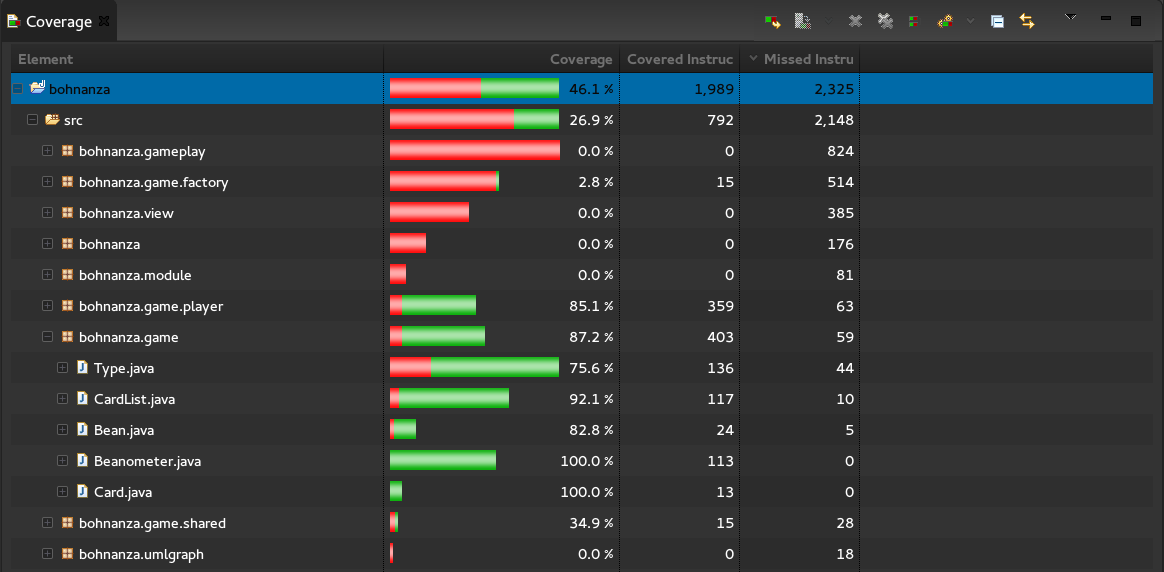
\includegraphics[width=\textwidth]{../img/coverage}
    \caption{Coverage of the \emph{bohnanza} module}
    \label{fig:test:coverage}
\end{figure}

\begin{figure}[h!]
    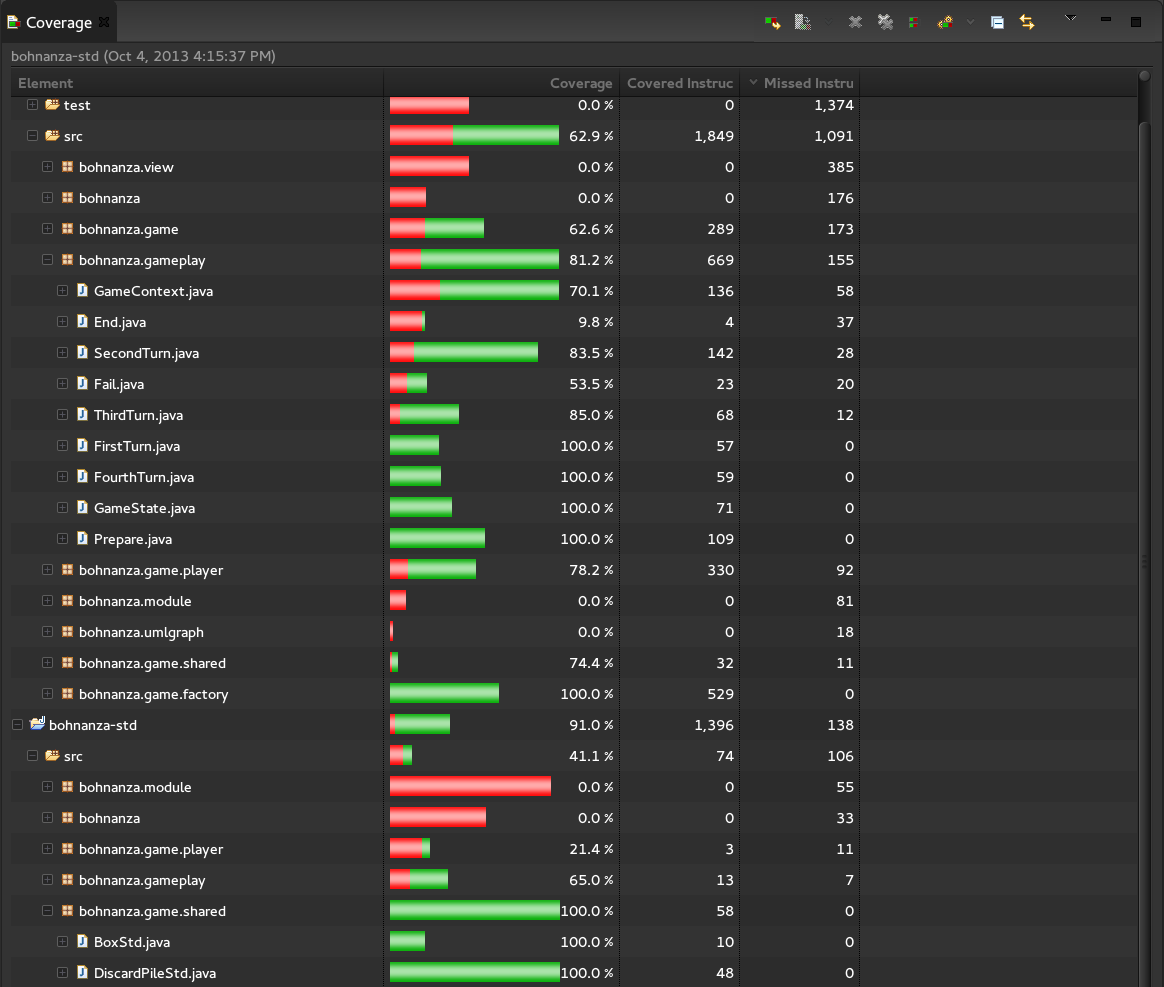
\includegraphics[width=\textwidth]{../img/coverage-std}
    \caption{Coverage of the \emph{bohanza-std} module}
    \label{fig:test:coverage-std}
\end{figure}
